\documentclass[notes]{subfiles}
\begin{document}
	\addcontentsline{toc}{section}{7.3 - Trigonometric Substitution}
	\refstepcounter{section}
	\fancyhead[RO,LE]{\bfseries \nameref{cs73}} 
	\fancyhead[LO,RE]{\bfseries \small \currentname}
	\fancyfoot[C]{{}}
	\fancyfoot[RO,LE]{\large \thepage}	%Footer on Right \thepage is pagenumber
	\fancyfoot[LO,RE]{\large Chapter 7.3}
	
\section*{Trigonometric Substitution}\label{cs73}
	\subsection*{Before Class}
	\addcontentsline{toc}{subsection}{Before Class}
	\subsubsection*{The Substitutions}
	\addcontentsline{toc}{subsubsection}{The Substitutions}
		\begin{ex}
			Use trigonometry to complete the following reference triangles: 
		\end{ex}
		\begin{center}
		\begin{tabular}{cp{.5in}cp{.5in}c}
			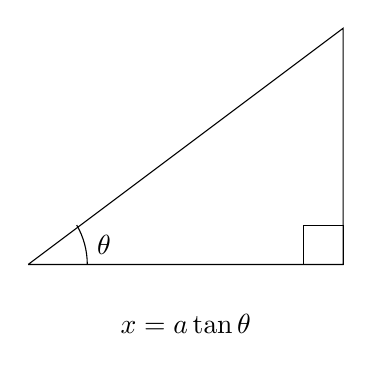
\begin{tikzpicture}
				\draw (0,0)--(4,3)--(4,0)--(0,0);
				\draw (.75,0) arc (0:30:1);
				\draw (.75,.25) node[right] {$\theta$};
				\draw (3.5,.5) rectangle (4,0);
				\node at (2,-.75) {$x = a\tan\theta$};
			\end{tikzpicture}
			& &
			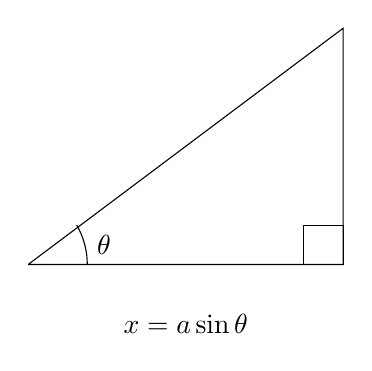
\begin{tikzpicture}
				\draw (0,0)--(4,3)--(4,0)--(0,0);
				\draw (.75,0) arc (0:30:1);
				\draw (.75,.25) node[right] {$\theta$};
				\draw (3.5,.5) rectangle (4,0);
				\node at (2,-.75) {$x = a\sin\theta$};
			\end{tikzpicture}
			& &
			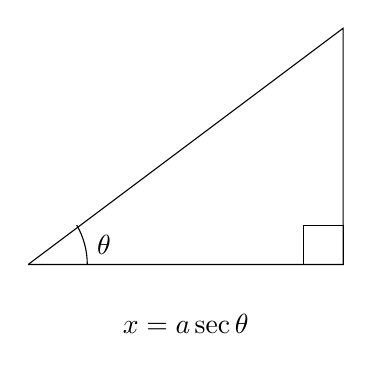
\begin{tikzpicture}
				\draw (0,0)--(4,3)--(4,0)--(0,0);
				\draw (.75,0) arc (0:30:1);
				\draw (.75,.25) node[right] {$\theta$};
				\draw (3.5,.5) rectangle (4,0);
				\node at (2,-.75) {$x = a\sec\theta$};
			\end{tikzpicture}
		\end{tabular}
		\end{center}
		
		\begin{ex}
			Let $f(x) = \dfrac{1}{16+x^2}$.
			\begin{enumerate}[(a)]
				\item Consider $\ds \int f(x)\, dx$.  Why do none of our previous integration techniques work here?
					\vs{1}
					
				\item Refer to the example at the top of the page.  Which triangle has an expression similar to the radicand in $f(x)$?  Write the substitution below.
					\vs{.5}
					\newpage
					
				\item Treat the substitution you chose in part (b) like a $u-$substitution.  Make the appropriate substitutions into the integral $\ds \int \dfrac{1}{16+x^2}\, dx$, and complete the integration.
					\vs{.75}
			\end{enumerate}
		\end{ex}
		
		\begin{ex}
			Compute $\ds \int \dfrac{\sqrt{9-x^2}}{x^2}\, dx$
		\end{ex}
			\vs{1}
		
		\begin{ex}
			Evaluate $\ds \int \dfrac{\sqrt{x^2-9}}{x}\, dx$
		\end{ex}	
			\vs{1}
			\newpage
			
	\subsection*{Pre-Class Activities}
	\addcontentsline{toc}{subsection}{Pre-Class Activities}
		\begin{ex}
			Use this space to write any questions you have from the videos.
		\end{ex}
			\vs{.5}
			
		\begin{ex}
			Compute $\ds \int_0^1 \dfrac{3}{x^2 + 4}\, dx$
		\end{ex}
			\vs{1}
			
		\begin{ex}
			Compute $\ds \int \dfrac{x}{x^2 - 4}\, dx$.  Is a trigonometric substitution necessary here?  Why or why not?
		\end{ex}
			\vs{1}
			\newpage
			
		\begin{ex}
			Compute $\ds \int \dfrac{1}{x^2\sqrt{4-x^2}}\, dx$ using the substitution $x = 2\sin \theta$.
		\end{ex}
			\vs{1}
			
		\begin{question}
			Using the previous examples as guideposts, fill out the following table:
			\begin{center}
			\begin{tikzpicture}
				\draw (-4,5) node[above]{\textbf{If you see an integrand involving}};
				\draw (4,5) node[above] {\textbf{Try a substitution using}};
				\draw (-8,5)--(8,5);
				\draw[thick] (0,5.5)--(0,-3);
			\end{tikzpicture}
		\end{center}
		\end{question}
			\newpage
			
	\subsection*{In Class}
	\addcontentsline{toc}{subsection}{In Class}
	\subsubsection*{Examples}
	\addcontentsline{toc}{subsubsection}{Examples}
		\begin{ex}
			Compute $\ds \int \dfrac{dx}{x^2\sqrt{x^2 + 9}}$
		\end{ex}
			\vs{1}
			
		\begin{ex}
			Evaluate $\ds \int_0^{3\sqrt{3}/2} \dfrac{16x^3}{(4x^2+9)^{3/2}}\, dx$
		\end{ex}
			\vs{1}
			\newpage
			
		\begin{ex}
			Compute $\ds \int \dfrac{\sqrt{x^2-1}}{x^4}\, dx$
		\end{ex}
			\vs{1}
			
		\begin{ex}
			Find $\ds \int \dfrac{x}{\sqrt{3-2x-x^2}}\, dx$
		\end{ex}
			\vs{1}
			\newpage
			
		\begin{ex}
			Evaluate $\ds \int \dfrac{dx}{(x^2-1)^{3/2}}$
		\end{ex}
			\vs{1}
			
		\begin{ex}
			Show that $\ds \int_0^a x^2\sqrt{a^2-x^2}\, dx = \dfrac{\pi}{16}a^4$
		\end{ex}
			\vs{1}
			\newpage
			
		\begin{ex}
			Evaluate $\ds \int \sqrt{x^2 + 2x}\, dx$
		\end{ex}
			\vs{1}
			
		\begin{ex}
			Compute $\ds \int \dfrac{x}{\sqrt{x^2 + 1}}\, dx$
		\end{ex}
			\vs{1}
			
		\newpage
	\subsection*{After Class Activities}
	\addcontentsline{toc}{subsection}{After Class Activities}
		\begin{ex}
			Use trig substitution to prove that the area of the ellipse $\dfrac{x^2}{a^2} + \dfrac{y^2}{b^2} = 1$ is $\pi ab$, where $a$ is the length of the major axis and $b$ is the length of the minor axis. 
		\end{ex}
			\vs{1}
			
		\begin{ex}
			Compute $\ds \int x^2\sqrt{3+2x-x^2}\, dx$
		\end{ex}
			\vs{1}
			\newpage
			
		\begin{ex}
			Evaluate $\ds \int_{\sqrt{2}/3}^{2/3} \dfrac{dx}{x^5\sqrt{9x^2-1}}$
		\end{ex}
			\vs{1}
			
		\begin{ex}
			Compute $\ds \int_0^1 \sqrt{x-x^2}\, dx$
		\end{ex}
			\vs{1}
	
\clearpage
\end{document}